\subsection{Ontology Management}\label{ssec:UseCase1-Ontology Management}

Each of the following two use cases apply a different ontology (i.e., \acrshort*{FOAF} and \tracknshrink{UNESCO}) to demonstrate two ways a user can approach this scenario. To manage the ontologies by a particular status, both scenarios use the property \acrshort{vs}\texttt{term\_status}, which values indicate \textit{“the status of a vocabulary term, one of ‘stable’, ‘unstable’, ‘testing’ or ‘archaic’”} \parencite{Miller2014}.

\subsubsection{Use Case 1: Update a FOAF Term Status}

In this use case, the \textit{\acrlong*{FOAF}} (\acrshort*{FOAF}) ontology acts as the underlying graph.\footnote{\acrshort*{FOAF} describes \textit{``[\textellipsis{}] persons, their activities and their relations to other people and objects [\textellipsis{}]''} \parencite[9]{Gargouri2010}. The ontology was created in mid-2000 by \textcite{Miller2014}. \acrshort*{FOAF} Homepage: \url{http://www.foaf-project.org/}.} Throughout this scenario, the current specification will be used for reference: \url{http://xmlns.com/foaf/spec/}.

\vspace*{\baselineskip}

\noindent \textsc{Outline}\\
\noindent \acrshort*{FOAF} terms can describe individuals in various ways. For example, terms like \acrshort{foaf}\texttt{name}, \acrshort{foaf}\texttt{depiction}, and \acrshort{foaf}\texttt{knows}, are typically used to describe individuals by their name, photo, and relations to other individuals. Each term contains several properties, and one property shared by all terms is \acrshort{vs}\texttt{term\_status}. For example, the term \acrshort{foaf}\texttt{mbox} (describing a personal mailbox) has a status value of \textit{stable},\footnote{Compare \url{http://xmlns.com/foaf/spec/\#term\_mbox}.} while the status value of \acrshort{foaf}\texttt{depiction} is \textit{testing}.\footnote{Compare with \url{http://xmlns.com/foaf/spec/\#term\_depiction}.}

Regarding the current use case, the first goal is to visualize all \acrshort*{FOAF} terms distributed over the board’s columns, depending on their inherent status value. The second goal is to change a term’s status value by dragging a card (i.e., a \acrshort*{FOAF} term) to another column. The user can easily change the status of the \textit{depiction} resource from \textit{testing} to \textit{stable} by dragging the corresponding card. This will trigger a graph update, that makes changes persistent.

\vspace*{\baselineskip}

\noindent \textsc{Board Component Resources}\label{par:FOAF-BCR}\\[-1.5em]

\noindent \hangindent=1.7cm \textit{Cards.}\tabto{1.7cm} The \acrshort*{FOAF} terms are representing the cards of the board. Since the vocabulary definitions are written in \acrshort*{RDF}/\acrshort*{OWL} \parencite{Miller2014}, one could retrieve all \acrshort*{FOAF} terms (\textit{n} = 75) when using the following card classes: \acrshort{owl}\texttt{Class}, \acrshort{owl}\texttt{ObjectProperty}, and \acrshort{owl}\texttt{DatatypeProperty}.\\[-1.5em]


\noindent \hangindent=1.7cm \textit{Columns.}\tabto{1.7cm} To manage the status of a \acrshort*{FOAF} term, the property \acrshort{vs}\texttt{term\_status} will be used.\\[-1.5em]


\noindent \hangindent=1.7cm \textit{Lanes.}\tabto{1.7cm} To provide a clearer structure, \acrshort{rdf}\texttt{type} will be used to distribute all \acrshort*{FOAF} terms over the lanes of the board. Introducing lanes in this scenario affects the board’s structure, similar to the transition from board (B) to (B*) in \autoref{fig:Kanban Boards} on page \pageref{fig:Kanban Boards}.


\vspace*{\baselineskip}

\noindent \textsc{Card Component Resources}\\
\noindent The \acrshort*{FOAF} terms should represent the titles of the cards. For example, the label of the term \acrshort{foaf}\texttt{mbox} is \textit{personal mailbox}, and should be used as the card’s title. Moreover, all \acrshort*{FOAF} terms carry an \acrshort{rdfs}\texttt{comment} property along with a descriptive value. These values should be displayed below the card’s title to provide more context to the user. For example, the descriptive text for term \acrshort{foaf}\texttt{mbox} is: \textit{“A personal mailbox, ie. an Internet mailbox associated with exactly one owner, the first owner of this mailbox.”} (see the \acrshort*{FOAF} specification).


\vspace*{\baselineskip}

\noindent \textsc{Mockup}\\
\noindent \autoref{fig:RMB Use Case 1} provides a mockup of the \acrshort*{RMB} with the contents requested by the board component and card component resources above. For demonstration purposes, the mockup showcases only four \acrshort*{FOAF} terms (i.e., \textit{Document}, \textit{personal mailbox}, \textit{knows}, \textit{depiction}), including their corresponding description (see current specification for reference). Due to this limited sample size, the prototype will only reflect the content it is aware of. In other words, there are no columns values depicted for the statuses \textit{unstable} and \textit{archaic}, since no resources are containing these values within this small sample. To give users the possibility to create new columns from scratch, it would require a solution allowing to enter an arbitrary string literal. The text boxes in \autoref{fig:RMB Use Case 1} depict an exemplary solution of such a feature (i.e., the \textit{new column value} field).

Nevertheless, as stated in the outline, all resources have been allocated according to their inherent status value, resulting in a prototype consisting of two columns. Furthermore, the content is distributed over three lanes by their broader domain (i.e., \acrshort{rdf}\texttt{type}, as requested by the board component resources). Moreover, the user is be able to intuitively change a resource’s status value by placing a card into another column, as exemplarily demonstrated in \autoref{fig:RMB Use Case 1} for the term \textit{depiction}.


\begin{figure}[ht]
    \libertineLF
    \centering
    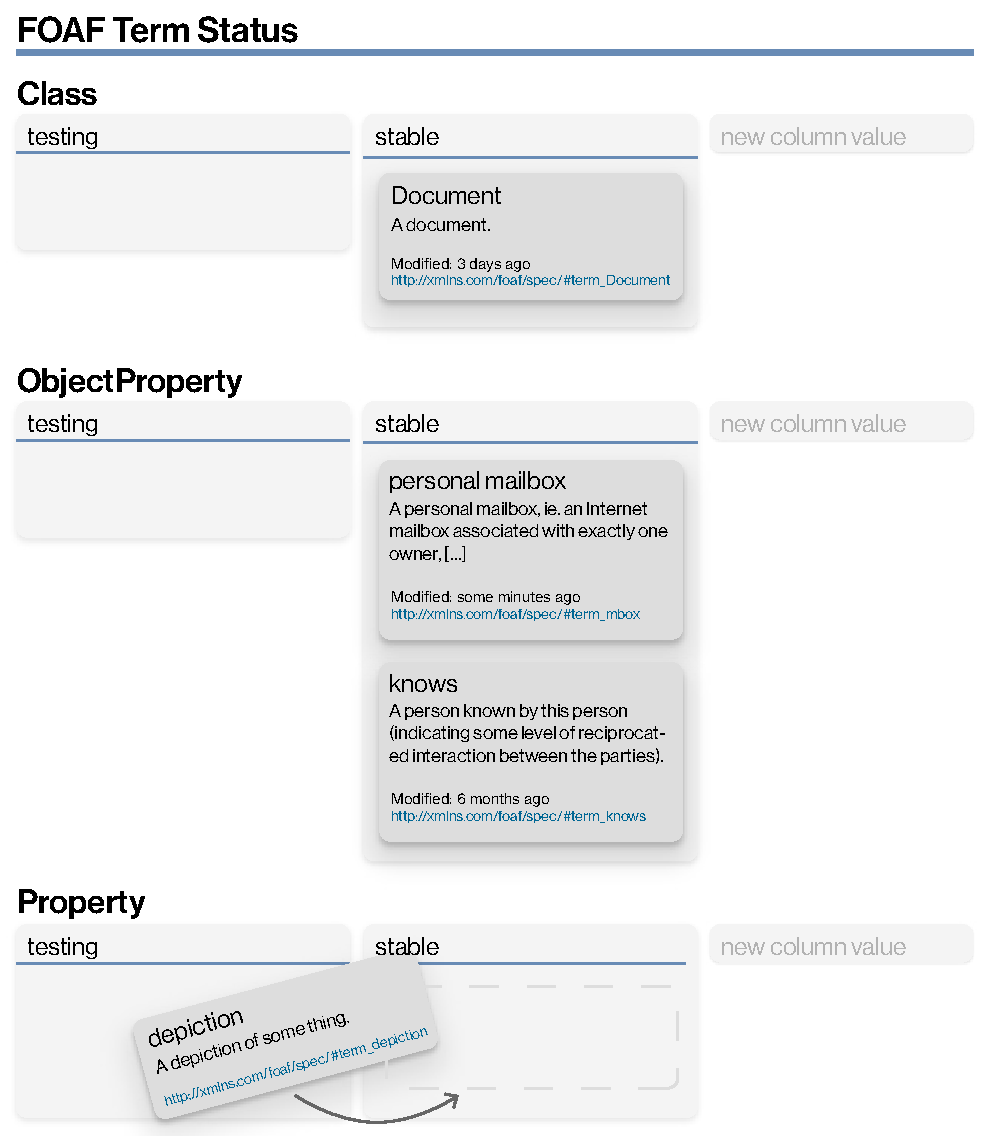
\includegraphics[width=142mm]{img/31-UseCase1.pdf}
	\caption[\tracknshrink{RMB} Mockup of Use Case 1]{\tracknshrink{RMB} Mockup of Use Case 1, showing a board that consists of two columns and three lanes grouping four \acrshort*{RDF} resources (i.e., \acrshort*{FOAF} terms). The resource \textit{depiction} is getting dragged into another column in order to update its current term status to the value \textit{stable}.}
	\label{fig:RMB Use Case 1}
	\libertineOsF
\end{figure}


\noindent Note that a timestamp does not only provide information about the last point of time a user moved a card. It also provides a visual cue to tell apart cards, that have been previously ‘touched’, from their untouched counterparts, as the latter ones lack a timestamp. For example, in \autoref{fig:RMB Use Case 1}, the resource \textit{depiction} has never been moved; thus, it does not contain a timestamp property. Eventually, when dropping the card, a timestamp gets generated, stored in the corresponding resource, and depicted on the card.